\documentclass{ctexbook}
\usepackage[
    paperwidth=185mm,
    paperheight=260mm,
    margin=25mm,
    top=30mm]{geometry}
\usepackage{footnote}
\usepackage{graphicx}
\usepackage{mdframed}
\usepackage{enumitem}
\usepackage{tocloft}
\usepackage{fancyhdr}

% \usepackage{tgpagella}
% \usepackage[U]{fontenc}

\usepackage{lecon-typographie}
% \usepackage{babel}

\CTEXsetup[number={\arabic{chapter}}]{chapter}
\setlength{\headheight}{13pt}

\pagestyle{fancyplain}
\renewcommand{\headrulewidth}{0pt}
\fancyhf{}
\fancyhead[LE, RO]{\thepage}
\fancyfoot{}

\fancypagestyle{plain}{
\fancyhead{}
\fancyfoot{}
}

\begin{document}

\frontmatter
\maketitle
\chapter*{注意}

在1990年,我写了一本名为《排版小课堂》的小书,其中收录了我在《Irisa周报》上以专栏形式发表的文章,我在其中“回顾”了一些排版的基本规则,并打算以此为基础编写一本科技文章写作手册。但我很快意识到这项工作的困难,甚至可以说是徒劳的,于是我就搁置了这个项目。

然而,《小课堂》被人以不太合法的方式(通常是盗版)上传到了网络上,并且格式不太便于访问(.dvi文件)。因此,有人要求我重新发布它们。在长时间的犹豫之后,我决定利用这个机会对它们进行重写、校对和扩充……在它们准备好之前,先放出这个版本——它在1990年原版的基础上做了轻微修改
    \footnote{主要的不同之处包括:版式、目录结构、增加了一些\emph{URL}、更新了参考文献……以及纠正了过去和未来的读者向我指出的一些录入错误(感谢读者们)。然而,我还没有增加任何补充内容,没有修改某些规则的表述,也没有重新审视我的某些原则选择来更贴近让-皮埃尔·拉克鲁(Jean-Pierre \textsc{Lacroux})的《正字法》(参见参考资料[\ref{ref5}],第~\pageref{ref5}~页)。%TODO
    }
。

我不能对那些被复制到其他网站上的版本的状态负责。只有本网站上的版本才能被视为最新版本:\link{http://jacques-andre.fr/faqtypo/lessons.pdf}
    \footnote{\emph{URL}、对参考资料的引用以及\textcolor{brown}{彩色}的脚注标记都是可点击的。}
。\label{aver}

\begin{flushright}
© 雅克·安德烈\\
© Jacques André\\
2003年10月版\\
此文档持续更新
    \footnote{以下人员提出了修正建议,在此一并感谢:\\
    Alem Alquier、Marwan Auger、Alain Bacquey、Guillaume Becq、Patrick Bideault、Stéphane Bortzmeyer、Guillaume Cabanac、Yves Cinotti、Antoine Colin、Pierre Dauchy、Armelle Domenach、Matthieu Dubuget、Laurent Douchin、Gilles Esposito-Farèse、Daniel Flipo、Alain Fossé、René Fritz、Fabien Galand、Xavier Gnata、Jean-Philippe Guérard、Henri Jabot、Michel Joubert、Charles Levert、Claude Lenormand、Vincent Lerouvillois、Jean-Baptiste Luciani、Jonathan Maurice、Olivier Miakinen、Geneviève Naud、Marc-André Oberholzer、Serge Paccalin、Patrick Percot、Olivier Pérès、Normand Perron、Éric Picheral、Jean-Baptiste Rouquier、Filippo Rusconi、Lionel de Sá、Arnaud Schmittbuhl、Gerhardt Stenger、Michel Taton、Patrice Tréton
    }
,最后一次更新是在2020年8月1日。
\end{flushright}

\vfill
\begin{center}
    \emph{发现法文原书的任何错误请反馈至:
    }

    Jacques.AndreNN@gmail.com\qquad 其中NN=35
\end{center}



\mainmatter
\chapter{为什么要开课?}

\paragraph*{先来个练习}让我们从下面这篇虚构的文章开始(不必关注它所涉的背景知识)。这篇文章包含了一些排印错误,或者说一些用法的错误 
    \footnote{不像拼写有正字法,法文没有官方的``排印规则'',取而代之的是建议、步骤等(参见第 \ref{chap8} 章的参考资料)。然而,尽管不同作者的用法不尽相同,这些用法之间也十分相似。可以说,一些用法已经达成了共识!}
。你能找到几处错误?

\begin{figure}
    \centering
    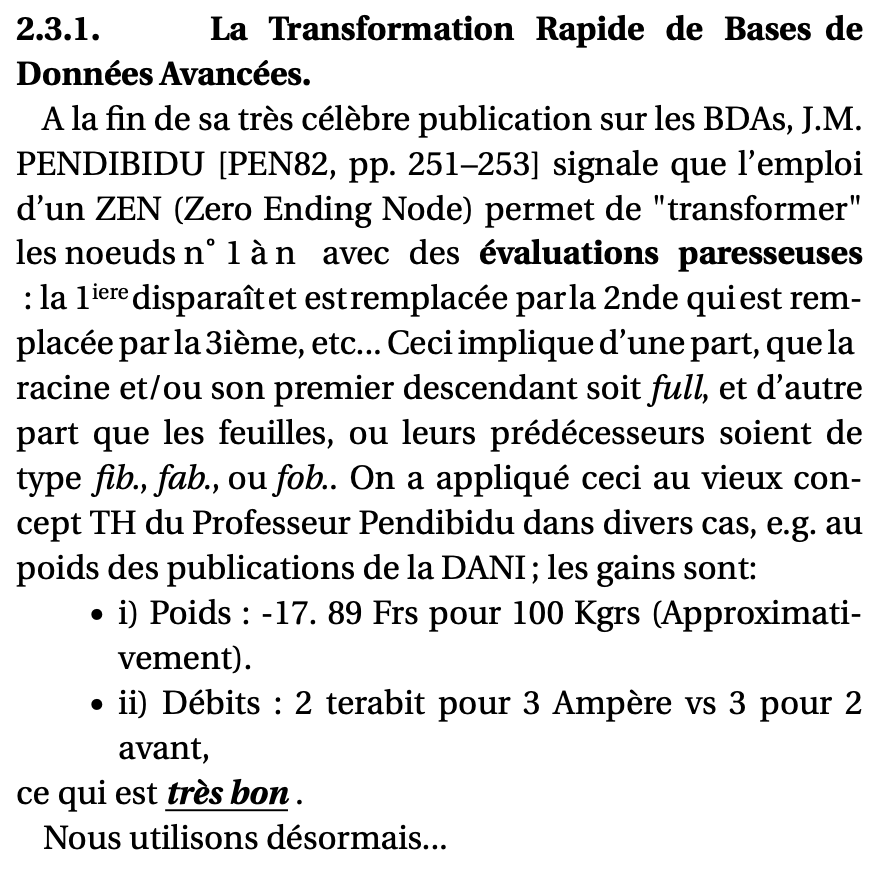
\includegraphics[width = \linewidth]{img/1.png}

\begin{mdframed}
    \footnotesize
    \textbf{2.3.1 \quad 高级数据库的快速转换.}\\
    J.M. PENDIBIDU [PEN82, pp. 251-253]在其关于BDAs的著作的结尾指出,使用ZEN(Zero Ending Node)可以通过\textbf{懒评估}来\verb|"|转换\verb|"|节点n° 1到n:
    1$^{\rm iere}$消失了,被2nde取代,而2nde又被3ième取代,等等……
    这一方面意味着根和/或它的第一个后代为\emph{full},另一方面意味着叶节点或其前代的类型是\emph{fib.}、\emph{fab.}或\emph{fob.}.
    我们在不同的情况下将其应用于Pendibidu教授的旧概念TH,例如DANI的出版物重量;结果如下:\\
    $\cdot$ i) 重量:-17. 89 Frs每100 Kgrs(约).\\
    $\cdot$ ii) 流量:对于3安培为2太位vs之前为3、2,\\
    这种结果\textbf{\emph{\underline{非常好}}}.\\
    现在,我们用……
\end{mdframed}

    \caption{组织得很糟糕的文字}
    \label{fig1}
\end{figure}

如果你将这样的文章直接发给仍然带有编辑部门的学术期刊,如《信息科学技术》(\emph{Technique et Science Informatiques,TSI}),你将收到如图\ref{fig2}所示的校样,并且期刊会要求重新整理稿件。

\begin{figure}
    \centering
    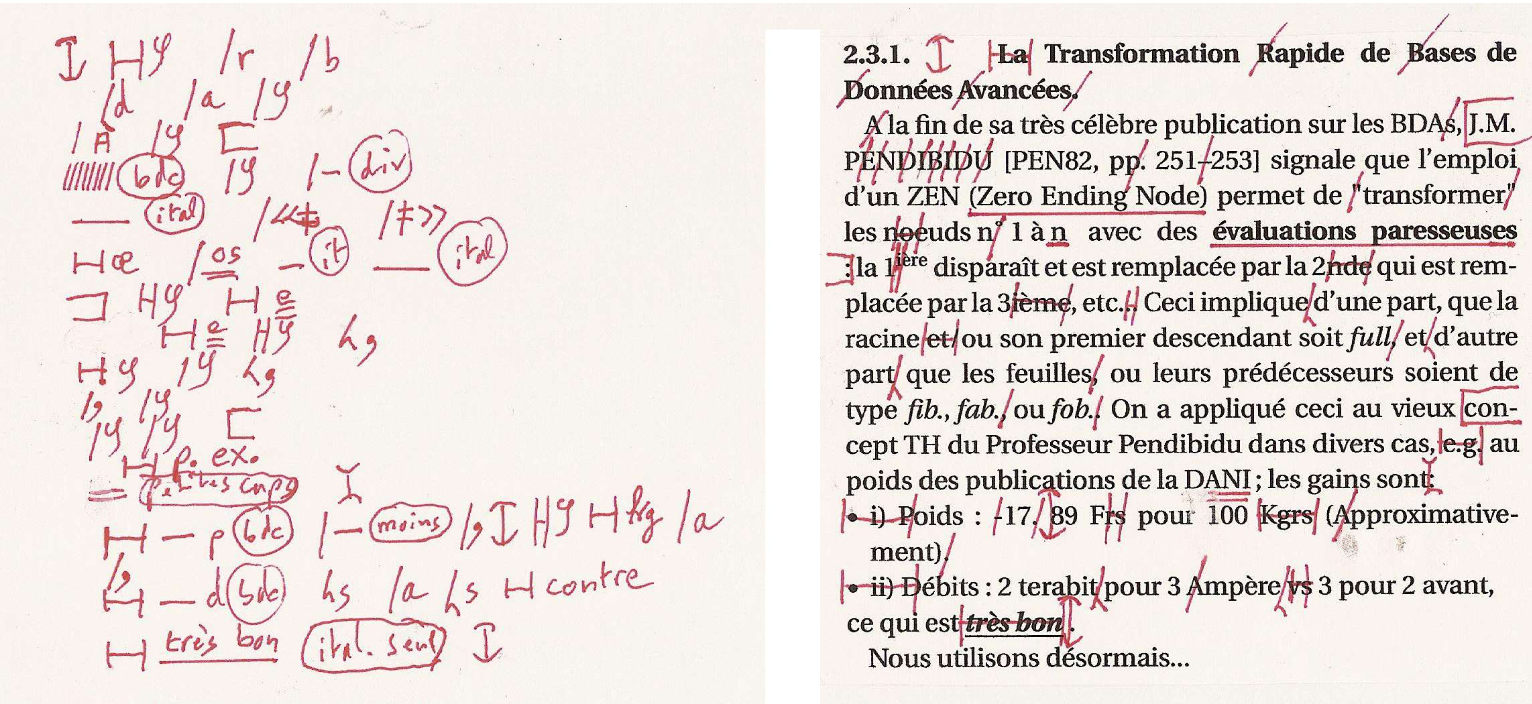
\includegraphics[width = \linewidth]{img/2.png}
    \caption{图\ref{fig1}中的文字,带有校对符号}
    \label{fig2}
\end{figure}

在这里,我们不会为你提供上面练习的详细解答,因为它会非常长。但我们会在下面列出一些具有代表性的差错(校对标记就代表了差错,其更正形式见图\ref{fig3}),并在图\ref{fig3}中以更好的方式呈现了这一小段文字。图\ref{fig1}中的文字有以下经典错误:

\begin{itemize}
    \item 标题:
    \begin{itemize}
        \item 标题一般不加冠词;
        \item 标题不采用各单词首字母大写的形式;
        \item 标题结尾不加句点。
    \end{itemize} 
    \item 第1行:
    \begin{itemize}
        \item 大写字母应当添加变音符号(见\ref{sec3.2}节);
        \item 首字母缩写不应带复数(见\ref{sec2.3}节);
        \item 不在姓名中间换行(见\ref{sec5.1.3}小节)。
    \end{itemize}
    \item 第2行:
    \begin{itemize}
        \item 专有名词不应全大写;
        \item 表示页码的缩写应当是``p.''(见\ref{sec2.3}节)。
    \end{itemize}
    \item 第3行:
    \begin{itemize}
        \item 外语单词连带其两侧的圆括号应当设为意大利体(见\ref{sec4.6}节);
        \item 法文的引号应当为双楔形的«...»形式(见\ref{sec2.2}节)。
    \end{itemize}
    \item 第4行:
    \begin{itemize}
        \item noeud的正确拼写形式应当为nœud;
        \item numéro的缩写应当使用上角字母o(n$^{\rm o}$)而此处使用了度的符号(n°),且需要添加代表复数的$^{\rm s}$。
    \end{itemize}
    \item 第5行:
    \begin{itemize}
        \item 冒号应当位于上一行;
        \item 第1和第3的缩写应当分别为$1^{\rm re}$和$3^{\rm e}$(见\ref{sec2.3}节),但最好是写出全称,且此处的seconde应当使用deuxième。
    \end{itemize}
    \item ……
\end{itemize}

\begin{figure}
    \centering
    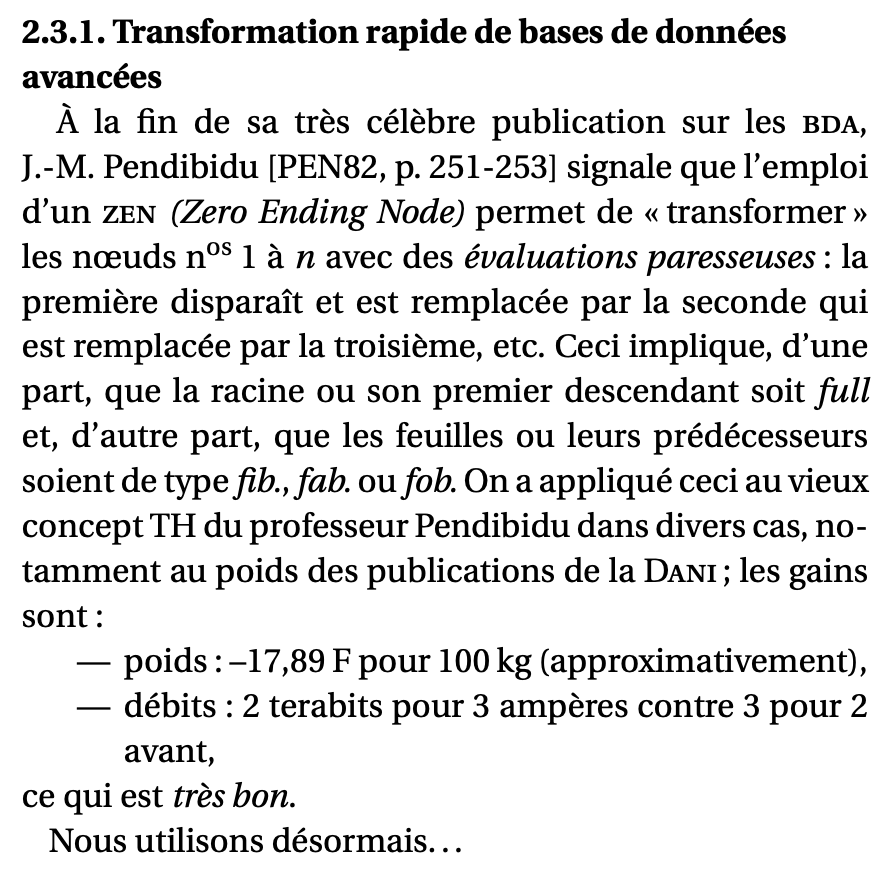
\includegraphics[width = \linewidth]{img/3.png}

\begin{mdframed}
    \footnotesize
    \textbf{2.3.1 \quad 高级数据库的快速转换}\\
    J.M. Pendibidu [PEN82, p. 251-253]在其关于\textsc{bda}的著作的结尾指出,使用\textsc{zen}\emph{(Zero Ending Node)}可以通过\emph{懒评估}来«转换»节点n$^{\rm os}$ 1到$n$:
    第1个节点消失了,被第2个取代,而第2个又被第3个取代,等等。
    这一方面意味着,根或它的第一个后代为\emph{full},另一方面意味着,叶节点或其前代的类型是\emph{fib.}、\emph{fab.}或\emph{fob.}。
    我们在不同的情况下将其应用于Pendibidu教授的旧概念TH,例如\textsc{Dani}的出版物重量;结果如下:\\
    \mbox{\qquad} ---  重量:$-17,89$ F每100 kg(约数),\\
    \mbox{\qquad} ---  流量:对于3安培为2太位,对比之前为3、2,\\
    这种结果\emph{非常好}。\\
    现在,我们用……
\end{mdframed}

    \caption{与图\ref{fig1}相同的文字,合入图\ref{fig2}的校对符号}
    \label{fig3}
\end{figure}

按理说
    \footnote{我使用了这个短语的现代写法:À priori。见\ref{sec4.6}}
,我们想指出,这并不是在钻牛角尖(尤其是已经攒了这么多出来)。然而,看看修改过的版本(图\ref{fig3})就可以发现,文本更可读了、表达更精准了。遵循这些排印规则不需要什么成本,去了解和应用它们也是如此。

然而,为什么会出现这么多错误呢?事实表明,研究人员越来越多地自己撰写文章或报告,可是他们很少接受的文书方面的培训,也就会经常忽略拼写和排印错误。此外,科技出版在过去(实际上也没有过去多少年),不论是从内容是形式上讲,都出自专业之手——内容上,有期刊编辑委员会、大会科学委员会等来把关;形式上,有文字编辑部门来把关——不像今天,任何人都可以通过\emph{网络}来随便写些什么东西。在那样的形势下,完好呈现出来的文件,无论是印刷品还是显示在屏幕上,实际上都在发行之前被掘地三尺地编校过。例如,在IRISA(Institut de Recherche en Informatique et Systèmes Aléatoires,计算机科学和随机系统研究所)1989年的活动报告中,平均每页被找出6个差错。至于硕士生写出来的大小论文……好吧,这些作者都已经有一些排印(typographie)的基础知识了
    \footnote{或者说\emph{正字法(orthotypographie)}知识,除了字体、版式等内容外,还包含了使用正确的正字符号,而这也是排印的一部分。}
。

这个小课堂的目的是促使我的同事
    \footnote{鉴于他们都是计算机科学家或自动化专家,我的例子往往更贴这些领域。}
更好地把控他们的出版物中的文字,以提升其质量。

以下所有内容都与任何排版引擎无关
    \footnote{尽管我认为\LaTeX (也就是这个文档所使用的排版引擎)对于科技文本来说更适合,无论针对纸质内容还是\emph{网络}内容,但我还是要指出,有个东西叫MS Word。}
,也不涉及任何美观的问题(如何选择字体、如何选择布局等,见参考文献)%TODO
。最后,这些内容同时适用于印刷和屏幕显示。
\chapter{来写点高质量法文如何?}

研究人员越来越多地被要求使用英文来写作文章、报告等,去适应美国英语的规则(见参考资料%TODO
)。

但是,仍然有大量的情况允许我们或需要我们去使用法文,或者说,用正确的法文写作。如果说一些``规则''存在,那它们的目的就不是给你添堵,而是让文字更易懂、更易读。``写法文''包含

\begin{itemize}
    \item 遵循法文的拼写规则和语法,
    \item 以及使用正确的法文排印符号、适宜的缩写,等等。
\end{itemize}

其中,第一点不是本\emph{排印}小课堂的内容,但我想着重指出,现在可以找到五花八门的拼写检查工具,如MS Word集成的拼写检查功能、Ispell(法化版)等。

\begin{enumerate}
    \item 最大化使用这些工具,因为错别字总是让我们防不胜防。
    \item 充分了解它们的局限性:
    \begin{itemize}
        \item 它们通常会按照自认为正确的形式(字典上收录的形式)来纠正拼写,很少会考虑到性数配合;文章即使在MS Word上不被任何下线标红,也可能有很多配合上的问题。
        \item 最大化使用自定义词库来避免文中使用的科技术语不被识别或``被改错
            \footnote{我曾在一个科技小论文上见过一台``快到基于12年一次的循环的计算机'',MS Word无法识别纳秒(ns),将其改为了年(ans)!}
        ''的情况。
    \end{itemize}
\end{enumerate}

\section{法文字母}

今天的法文字母表包含42个(而不是26个)字母:

\begin{center}
    \Large a b c d e f g h i j k l m n o p q r s t u v w x y z \\
    à â é è ê ë î ï ô ù û ü ÿ ç æ œ
\end{center}

法文中,带有重音符的\emph{u}只在\emph{où}这一个单词中出现;带有分音符的\emph{u}很少出现
    \footnote{在aiguë、ambiguïté、contiguë等词中,分音符不出现在\emph{u}上,而是出现在其后紧随的元音上。}
,只在古法文或外来词(如capharnaüm、Bienvenüe等)中出现。带有分音符的\emph{y}(\emph{ÿ})出现在专有名词(L'Haÿ-les-Roses)或专有名词的派生词(aÿ,一种香槟)中。\emph{Œ}和\emph{œ}不是简单出于美学考虑的合字,我们不能统一将\emph{oe}替换成\emph{œ}(请想想``nœud coercitif''[强制节点]这个词组)。字母表中带有双字母\emph{æ}(罗马体写作æ),这是因为它在一些外来词(ægagropile、philæ等)或地名中出现。

请注意,法文中没有\emph{ñ}和\emph{ö},即使一些法文字典开始收录了cañon、angström、maelström等词。

每个字母都可以以3种形式使用,比如``aA\textsc{a}'',这代表:

\begin{enumerate}
    \item 小写(minuscule,也称作bas de casse)形式,如abéçô。
    \item 大写(majuscule,也称作capitale)形式,如ABÉÇÔ。
    \item 小型大写形式。简单来说,是看起来像大写字母的小写字母——\textsc{abéçô}。它用于表示首字母缩写、参考资料中的作者姓,以及一些结构上的元素(戏剧的对话、法律条文等)。
\end{enumerate}

变音符号在法国文化中占据一席之地,使用它们是非常重要的。哎呀,我们不是总能在打字机或计算机的键盘上``直接''找到这些字符(例如,我们通过\^{}\emph{o}来打出\emph{ô},至于\emph{É}嘛……)。字库中收纳了所有这些法文字符,没有任何理由不去使用它们(除了蠢和懒)。

\paragraph*{练习} 使用你喜欢的文字处理软件输入下面的全字母句
    \footnote{这句话由吉勒·埃斯波西托-法雷塞(Gilles Esposito-Farèse)设计。全字母句是指包含给定语言中的所有字母的句子,且长度越短越好。有一本C语言手册中用英文给出了这样一个示例:\texttt{char *MyString = "The quick brown fox jumps over the lazy dog";}。译者显然什么都不懂,直接将其翻译成了\texttt{char *ZiFuChuan = "那只敏捷的棕毛狐狸跃过那只懒狗";}。想要在法文中保留全字母句,至少也应当翻译成\texttt{"Portez ce vieux whisky au juge blond qui fume"(把那杯老威士忌带给抽烟的金发法官)}……
    }
(先使用小写字母,再使用小型大写字母)。

\begin{center}
    Dès Noël où un zéphyr haï me vêt de glaçons würmiens\\
    je dîne d'exquis rôtis de bœuf au kir à l'aÿ d'âge mûr\\
    \& cætera !

    \textsc{Dès Noël où un zéphyr haï me vêt de glaçons würmiens\\ je dîne d'exquis rôtis de bœuf au kir à l'aÿ d'âge mûr\\ \& cætera !}
\end{center}

如果你做不到,必须去更换系统……

\section{一些排印符号}

文本不只包含字母、数字和标点(见第\ref{chap5}章),还包含一整套跟随语言而特定变化符号。以下是一些法文符号。

\begin{description}
    \item[法文引号] 在法文中,引号是一对双楔形符号«...»,而不是英文的\emph{(双)蝌蚪形符号}``...''或`...'(见图\ref{fig1}第5行)。
    \item[连接号] 我们要区分使用3种连接号:\\
    - 用于连词或行末\\
    -- 用于标示减号\\
    --- 用于标示插入语或列表元素,却有被中间的``--''取代的趋势。
\end{description}

相反地,以下符号需要避免:

\begin{description}
    \item[$\bullet$] 美国化符号,太粗大;需要使用--或---替代(见图\ref{fig1}第14行);
    \item[/] 这个斜杠被(过于)经常地作为``或''的含义使用;在文本中更倾向于使用连词``或''(ou),它只多占了一个字符。\\
    在什么情况下,我们都不用``或/和'' ``和/或''这样的表达,它们不比一个``或''字包含任何更多信息:在法文中,\emph{或}不是不相容的(见图\ref{fig1}第9行)。
\end{description}

\section{缩写}

一些缩写已经约定俗成,需要坚持使用下去,其中大多数不需要大写:用art.代表article,用vol.代表volume,等等。它们也不需要加复数后缀。但是,一些缩写的单数和复数形式不同(例如,M.代表monsieur,其复数messieurs的缩写为MM.),需要在行文中避免这样的缩写。以下是一些需要了解的常用缩写(可参阅任何排印语言良好的长列表,参阅参考资料%TODO
)。

\begin{center}
    \begin{tabular}{|l|l|}
        \hline
        artivle(文章/条款)& art.\\
        bulletin(通报)& bull.\\
        tome(卷)& t.\\
        page, pages(页,单复数)& p. \\
        numéro(序号,单数)& n$^{\rm o}$  N$^{\rm o}$ \footnotemark\\
        numéros(序号,复数)& n$^{\rm os}$ \\
        document(文档)& doc. \\
        édition(版)& éd.  \\
        sous la direction de(指导) & sld(英:\emph{ed.})\\
        et collaborateurs(等人)& et coll.(不用\emph{et al.})\\
        note de la rédaction(编者按)& n.d.l.r.\\
        \emph{confer}(= voir;参考)& cf.(用罗马体)\\
        c'est-à-dire(即)& c.-à-d.(不使用c.a.d或\emph{i.e.})\\
        Monsieur(先生)& M.  \\
        Madame(女士) & M$^{\rm me}$\\
        \hline
    \end{tabular}

    \footnotetext{上标使用字母而非度号}

\end{center}

\begin{center}
    \begin{tabular}{|l|l|l|}
        \hline
        形容词 & 缩写\footnotemark & 不要使用 \\
        \hline
        premier(第一,阳性单数)& 1$^{\rm er}$, 1er & 1$^{\rm ier}$, 1ier \\
        première(第一,阴性单数)& 1$^{\rm re}$, 1re & 1$^{\rm ière}$, 1ière, 1ere \\
        premières(第一,阴性复数)& 1$^{\rm res}$, 1res & 1$^{\rm ières}$, 1ières \\
        deuxième(第二)& 2$^{\rm e}$, 2e & 2$^{\rm ième}$, 2$^{\rm eme}$,  2ème, 2è \\
        \hline
    \end{tabular}
    
    \footnotetext{在极少数字母上标不可用的情况(如电子邮件)下,不使用上标的情况是可以容许的。}
\end{center}

\begin{center}
    \begin{tabular}{|l|l|}
        \hline
        副词 & 缩写\\
        \hline
        primo(首先) & 1$^{\rm o}$ \\
        secundo(其次) & 2$^{\rm o}$ \\
        tertio(其三) & 3$^{\rm o}$ \\
        quarto(其四) & 4$^{\rm o}$ \\
        \hline
    \end{tabular}
    
    \footnotetext{在极少数字母上标不可用的情况(如电子邮件)下,不使用上标的情况是可以容许的。}
\end{center}

\section{单位}

研究人员不知道怎么写测量单位——请你相信这个结论,我不想去费时费力地解释它。在这里,我只给出几个例子:2安培应当写作deux ampères,不应使用Ampère或Ampères,2~A的写法也是正确的;2,34~kg是正确的,2.34~Kilos是错误的,2,34~Kgrs更是错得离谱;17~F是正确的,17~Frs是错误的。请参阅参考资料%TODO
。

\section{断字}

行末单词的断字(称作coupure、césure或division[最后一种叫法更好些])的工作通常是由文字处理系统处理的,它们在多年前就已经在这方面取得了不少进展。但不论如何,它们偶尔还是会出些问题(见图\ref{fig1}第11行),甚至引入差错。因此应该由作者去确保断字正确,不要打断不该打断的单词。

然而,目前的文字处理系统很少能够处理单词间的断字问题,尤其是数字和紧随其后的单位间、人名首字母和姓之间不应换行(见\ref{fig1}第3行)。这就需要用到一个不可分空格(une espace
    \footnote{这里的espace是阴性名词。在铅字排印时期,这个词的阴性指能在一行文字间产生用于单词或符号的“空白”的一个字符。现在,即使字符已“去金属化”,法文仍然延续了这个用法,将能够产生空白的字符作为阴性名词使用。}
insécable;见\ref{sec5.1.3}小节)。

注意:在引用一段外文时,应当使用改文种的用法来确定断字规则。以下是一个例子:

\begin{quote}
    ……单词潜意识识别(英文称作\emph{word sub-\\
    liminal recognition})……
\end{quote}

\section{美国化}

受教于美国出版物,人们趋于相信其中的各种用法组成了一套自己的规则,并东施效颦,引入各种美国化的内容。然而,其中一些用法本有对应的法文。

\paragraph*{拉丁文短语} 以英语为母语的人笔下的那些短语,即使来源于拉丁文,也不符合法文的用法。

\begin{center}
    \begin{tabular}{|l|l|}
        \hline
        避免使用 & 使用 \\
        \hline
        \emph{e.g.} & p. ex. \\
        \emph{et alii, et al.} & et co-auteurs, et coll., etc.\\
        \emph{id est, i.e.} & c'est-à-dire, c.-à-d.\\
        versus, vs & contre, « - » \\
        \hline
    \end{tabular}
\end{center}

\paragraph*{缩写} 不同国家的缩写不同。例如:

\begin{itemize}
    \item 页(复数):法文使用p.,英文使用pp.;
    \item 先生:法文使用M.,英文使用Mr。
\end{itemize}

\paragraph*{正字法} 有很多区别,举例如下:

\begin{itemize}
    \item 标点符号(英文中,分号、冒号等符号前不加空格);
    \item 引号(英文为``...'',法文为« ... »);
    \item 法文中,标题的各实词首字母不需要大写,等等。
\end{itemize}

http://www.panamo.com/RESS/anglais.html 列出了很多其他区别。
\chapter{大写字母的作用}

\section{大写字母的滥用}

在阅读其他人写的科技文档时,最让我恼火的莫过于滥用大写字母。以下是一个典型的句子,出自我们的活动报告:

\begin{quote}
    Jean TRANSEN, Maître de Conférences en Analyse des \\
    Données à l'Université de Nancy (Bien connue de la Com-\\
    munauté Scientifique Internationale) a donné, lors du Sé-\\
    minaire de Biologie Informatique du Mardi 23 Juin, une \\
    conférence sur les Applications de l'Intelligence Artificielle \\
    à l'emploi de la Télévision Haute Définition en Robotique \\
    Avancée.

    \begin{bil}
        南希大学数据分析副教授让·特拉桑(国际科学界知名)在6月23日(星期二)的计算机生物学研讨会上就人工智能在高级机器人技术的高清电视中的应用发表了演讲。
    \end{bil}
\end{quote}
    
这句话中用了31个大写字母,而如果大小写规则应用正确,则只需要3个(只有Jean、Transen和Nancy需要大写)。没错,没错……我们将在\ref{sec3.6}节重新讨论这件事。

大写字母
    \footnote{在排印学中,我们将大写字母称为``capitale'',将小字写字母称为``bas de casse''。参见稍后的注释\ref{note15}。}
的使用充满了特殊情况,但我们可以依照如下的方法来为基本规则分类。在开始之前,再次强调,大写字母和小型大写字母都应该正确地带有变音符号。

\section{大写字母需要带变音符号吗?}

尽管我们在小学是可能(错误地)学过,大写字母不加变音符号,尽管一些编辑或期刊工作人员不会系统地处理变音符号
    \footnote{但会保持一致性。具体的原因(参见参考资料[3, 6]%TODO
    )跟语言学大写(majuscule)和排印学大写(capitale)有关。例如,VICTOR HUGO包含10个排印学大写字母,但只有2个是语言学的大写字母。}
,但下面这句话需要作为一条规则来遵守:在今天,没有任何理由来不为大写字母添加变音符号。相反,我们有太多地理由来为系统地添加变音符号。在这里给出了3个例子来证明带有变音符号的大写字母有助于文字的理解,实际上,还有更多例子能佐证这一点
    \footnote{有很多实用的例子(参见http://www.synec-doc.be/doc/accents2.htm)可以证明,使用小写字母(因为一些短语通常没有必要使用大写字母)或结合背景知识可以减少歧义。例如,SABLE SALE写在海滩入口的牌子上代表``沙子很脏''(sable sale),而写在饼干包装上代表``咸酥口味''(sablé salé)。相反,戏剧海报上写着CLAUDE S'EST TUE并不会减少歧义,可能是``克劳德自杀了''(Claude s'est tué),也可能是``克劳德沉默了''(Claude s'est tue)……}
:

\begin{enumerate}
    \item 在Minitel上发出以下消息的人收到了很多年长男性的打扰,因为很多人将``要求年龄相仿''(même âge)读成了``大龄人士也可''(même âgé):
    \begin{quote}
        CHOUETTE NANA, 18 ANS, CHERCHE MEC, MEME AGE, ... 
        \begin{bil}
            舒埃特·娜娜,18岁,寻找男士,要求年龄相仿……
        \end{bil}
    \end{quote}
    \item 在瑞士洛桑,有一条很陡的街道叫做le Petit-Chêne,在街道的入口有个牌子写着DANGER MARCHE(danger marche,行路危险/danger marché,危险集市)。看起来它只在周三起作用,因为周三才有集市。
    \item 本文档封面上的图片来自蒙帕纳斯的一家海鲜餐厅的招牌,上面的``海鳗''(le congre)是否写多了一个\emph{S}%TODO 封面
        \footnote{答案是没有。实际上,它写的是``议会''(le Congrès),只不过\emph{CONGRÈS}的\emph{È}缺了重音符。这里的背景知识没有给出:这家餐厅只是一家分店,而它的总店位于巴黎的Porte Maillot大道,靠近会议中心(Palais des congrès)。}
    ?
\end{enumerate}

如果你论文的指导老师认为,大写字母加不加变音符号只是个人喜好,请向他出示以下内容:

\begin{quote}
    « On veillera à utiliser systématiquement les capitales accentuées, y compris la préposition À. »\\
    \emph{Lexique des règles typographiques en usage à l'Imprimerie nationale}, Paris, 2004, p. 12.
    \begin{bil}
        ``注意,应始终使用带有变音符号的大写字母,包括介词À.''\\
        ——《国家印刷馆实用排版规则汇编》,巴黎,2004,第12页。
    \end{bil}
\end{quote}

\section{大写字母的几个作用}

\subsection{句子和括号}

这里有几个原则:

\begin{itemize}
    \item 句子的第一个字母应用大写,
    \item 插入语,尤其是以括号形式插入的内容不是句子,因此不以大写字母开头,
    \item 一般地,冒号后为小写字母。
\end{itemize}

举例如下:

\begin{description}
    \item[错误写法]  Ces transformations dépendent du type de nœud (Qu'il soit terminal ou pas) : Tant que...
    \item[正确写法] Ces transformations dépendent du type de nœud (qu'il soit terminal ou pas) : tant que...
\end{description}

\begin{bil}
    这些转换取决于节点的类型(无论其是否终端):只要……
\end{bil}

注意,美国人喜欢将注释整句放入括号,并且将其视为一句话。在法文中,没有理由这样做。举例如下:

\begin{description}
    \item[错误写法] ... et le temps d'exécution est négligeable. (On ne tient pas compte du cas où $v = 0$.) Si...
    \item[正确写法]  ... et le temps d'exécution est négligeable (on ne tient pas compte du cas où $v = 0$). Si...
    \item[更佳写法] ... et le temps d'exécution est négligeable ; on ne tient toutefois pas compte du cas où $v = 0$. Si...
\end{description}

\begin{bil}
    ……并且执行时间可忽略不计(且我们不考虑$v = 0$的情况)。如果……
\end{bil}

\subsection{文章及章节标题等}

\begin{itemize}
    \item 仅有标题的第一个字母需要大写。
\end{itemize}

举例如下(同时请参见图\ref{fig1}第1行):

\begin{description}
    \item[错误写法] Transparence de la Transmission de Message Asynchrone
    \item[正确写法] Transparence de la transmission de message asynchrone
\end{description}

\begin{bil}
    异步信息传输的透明性
\end{bil}

注意,前一个标题写得``美里美气''。

\subsection{列表}

大体上,我们可以将列表分为两类,一类一个独立句子的一部分,另一类本身就由多个句子组成:

\begin{enumerate}
    \item 在句子中的列表的元素以小写字母开始,以逗号(或分号)结束,除了最后一个元素要实用句点结束,因为同时作为句子的结尾;
    \item 由多个句子组成的列表的元素需要遵循单独段落的规则,即以大写字母开始,以句点结束。
\end{enumerate}

上面这个列表本身满足情况1(同时要注意,紧接数字的句点之后不需要使用大写字母)。除此之外,以下是两个其他例子:

\begin{quote}
    Les méthodes de déverminage sont basées sur
    \begin{itemize}
        \item la récolte d'événements~;
        \item la sauvegarde de l'état du programme à intervalles réguliers~;
        \item l'intégration des tâches au programme~;
    \end{itemize}
    mais on aurait une autre classification en se plaçant du point de vue utilisateur.
    \begin{bil}
        清理方法基于:
        \begin{itemize}
            \item 事件的收集;
            \item 程序状态的定期保存;
            \item 程序中任务的纳入;
        \end{itemize}
        但换到用户的视角,则有另一种分类方法。
    \end{bil}
    
\end{quote}

\begin{quote}
    Deux types d'événements sont à considérer.
    \begin{itemize}
        \item Les événements prédéfinis. La trace en est générée par le noyau.
        \item Les événements utilisateur. L'heure, par exemple, sera associée à l'événement en question.
    \end{itemize}
    Une fois stockés sur fichier, ces événements...
    \begin{bil}
        需要考虑两种事件:
        \begin{itemize}
            \item 预定义事件。其轨迹由内核生成。
            \item 用户事件。例如,时间需要与所涉及的事件相关。
        \end{itemize}
        一旦存储为文件,这些事件……
    \end{bil}
\end{quote}

\subsection{首字母缩略词}

这里说的更多是目前的趋势,而不是死规则:

\begin{itemize}
    \item 首字母缩略词中间不再总要加句点,
    \item 需要尊重首字母缩略词拥有方的使用习惯(尤其是否在大写字母上加变音符号),
    \item 在首字母缩略词可以整体发音时,仅将第一个字母大写,
    \item 如果首字母缩略词需要我们逐字母读出,则更偏向于使用小型大写字母,
    \item 一些首字母缩略词有时会构成徽标(比如法国电力集团[Électricité de France]的徽标是EDF而非\textsc{Édf}),我们遵从徽标上的写法,一些品牌名也如此(如iPod)。
\end{itemize}

以下是一些例子:Irisa、Ifsic、\textsc{Sncf}、EDF、\textsc{Cee}、Afcet、Greco、Sorep,等等。

\section{大写字母的语义学作用}

目前为止,规则都只受制于单词的位置和一些缩写的约定。滥用大写字母的一个原因是认为大写字母可以由强调或区分语义的作用。实际上,强调和区分语义应当交由其他排印学方式来完成(如使用意大利体)。

基本的规则如下。首字母大写可以表示

\begin{itemize}
    \item 专有名词,
    \item 跟专有名词等价的名称,
    \item 一定程度的尊重(用于客套)。
\end{itemize}

\subsection{专有名词}

\begin{itemize}
    \item 首字母大写。
\end{itemize}

但是,只有首字母应当大写。因此,应当写J.-M. Pendibidu或Jean-Marie Pendibidu,而不要写J.M. PENDIBIDU(见图\ref{fig1}第4行)。在文章标题中或作为参考书目时,我们倾向于使用小型大写字母来表示作者的姓,如Donald \textsc{Knuth}。

类似地,假名(如Raphaël le Tatoué[纹身人拉斐尔])、地名(如la Picardie septentrionale[北皮卡第大区])、非通用的商品名(如Bull vend des klaxons à Renault pour ses jeeps[公牛向雷诺出售吉普车喇叭])等也可以大写。

可以参与构成名称的冠词也使用大写,如les œuvres de La Fontaine(拉封丹的作品)。

\subsection{跟专有名词等价的名称}

这里需要区分3种情况:

\begin{enumerate}
    \item 标明独特性的普通名词(如la Bibliothèque nationale [国家图书馆]是唯一的;类似地,la Culture [文化部]表示一个部门而非宽泛的文化概念)可以看作专有名词,使用大写。当形容词对名称起到限定作用时,在名词前的形容词使用大写(如le Nouveau Monde [新世界]),在名词后的形容词使用小写(如l'Empire romain [罗马帝国])。
    \item 如果独特性是由专有名词表达的,则只有专有名词使用大写,其他单词使用小写:la bibliothèque d'Alexandrie(亚历山大图书馆)、la bibliothèque Mazarine(马萨林图书馆)。
    \item 一些普通名词可以作为专有名词使用,尤其是交通工具或作品名(这两种名词需要使用意大利体),如\emph{La Belle Poule}(贝勒·普尔[本义为美丽母鸡]号护卫舰)、\emph{Les mains sales}(戏剧《脏手》;对于这种情况,只有第一个冠词的首字母大写),以及节日名(如le Mardi gras [狂欢节,本义为油腻星期二])、政党或其他组织名(如le Parti communiste français[法国共产党];需要符合其措辞要求)等。
\end{enumerate}

所有的排印手册对会给出一系列不同情况的列表,但无疑更重要的是要注意\emph{不需要大写的情况}!参见\ref{sec3.5}节。

\subsection{出于礼貌或尊敬的大写}

\begin{itemize}
    \item 出于礼节,需要使用大写。
\end{itemize}

示例如下:Croyez, Cher Monsieur, en l'expression...(请相信,亲爱的先生,有句话……)

\section{延伸}

对于前文没有提到的情况,不使用大写字母。尤其是以下情况:

\begin{itemize}
    \item 不唯一的组织,无论是不是国有的,都不大写:l'université de Rennes(雷恩大学)、l'académie de Poitiers(普瓦捷学院)、 le conseil municipal de Rezé(雷泽市议会)、l'observatoire de Meudon(默东天文台)、la mairie de Paris(巴黎市政厅)等;有时我们将其视作法律实体或机构,此时则倾向于使用大写:... l'Université de Rennes-2 a décidé...(……雷恩二大决定……);
    \item 星期和月份不大写:mardi 25 janvier(1月25日星期二);
    \item 头衔或身份使用小写字母: le président de la République(法国总统)、le pape(神父)、l'ayatollah Khomeini(阿亚图拉霍梅尼)、le professeur Dupond(迪蓬教授)、le recteur Durand(迪朗院长)、le général Avendre(阿文德将军)、le ministre de l'Éducation nationale(教育部长)等
        \footnote{请看看《世界报》是怎么报世界的。跟人们普遍的看法相反,通常来说,报刊可以很好地应用法文排版,即使是地区报刊。}
    。
\end{itemize}

\section{回到第一个例子}

现在回看下本章开头提到的例子(见\ref{sec3.1}节)。

\begin{description}
    \item[Jean TRANSEN(让·特拉桑)] Jean的写法是错误的,但Transen只需要首字母大写,其他都是累赘。
    \item[Maître de Conférences(副教授)] 错。头衔不需要大写。这里只用``区分'',不用``尊敬''。
    \item[Analyse des Données(数据分析)] 错。如果迫不得已,我们要将其作为一个概念来区分这个学科,Analyse des données这样的写法是可以勉强接受的。对于更老一些的学科,人们都习惯了使用小写字母,如mécanique quantique(量子力学)或histoire de l'art(艺术史)。难道学科新就能理所当然地用大写字母吗?
    \item[Université de Nancy(南希大学)] université不需要大写,组织不是唯一的。当然,Nancy需要大写。
    \item[Bien] 括号内不需要大写。
    \item[Communauté Scientifique Internationale(国际科学界)] 这里也没有任何理由使用大写字母。
    \item[Séminaire de Biologie Informatique(计算机生物学研讨会)] 错。应该写séminaire de biologie informatique。迫不得已时,可以写Biologie informatique,就像Analyse des données一样。
    \item[Mardi 23 Juin(6月23日星期二)] 日期不用大写:mardi 23 juin。
    \item[Applications(应用)] 如果是引用会议的标题,那么标题应当首字母大写并且使用意大利体(作品名)或置于引号内;否则,不需要使用大写的A。
    \item[Intelligence Artificielle(人工智能)] 错。应该写intelligence artificielle。迫不得已时,可以写Intelligence artificielle。如果它的缩略语IA广为人所知,也可以直接缩略为IA。相反,则可以用大写字母来给出缩略语的说明:IA (Intelligence Artificielle)。
    \item[Télévision Haute Définition(高清电视)] 同上:应当写télévision haute définition或Télévision haute définition。当然,也可以写作\textsc{Tvhd}或TVHD (TéléVision Haute Définition)。
    \item[Robotique Avancée(高级机器人技术)] 还是一样的问题(不过至少这段文字逻辑通畅)……
\end{description}

我们需要证明并接受这些新规矩的存在。然而,还是有十多个多余的大写字母。也就是说,这短短7行文字中仍然有15处法文错误。

\section{第二个例子}

10月1日,一纸文件在雷恩的一些小学流传,上面这样写道:

\begin{quote}
    \emph{Le Conseil d'école réunit les représentants de L'Education Nationale et de la Municipalité, les Instituteurs et les parents.}
    \begin{bil}
        学校理事会由教育部和市政府代表、教师和家长组成。
    \end{bil}
\end{quote}

当然,除了表示教育部的\emph{Éducation}(教育)和句子开头外,本不该出现任何一个大写字母。我们可以容忍\emph{le Conseil d'école}(学校理事会)的写法,它是唯一的,而到了\emph{la Municipalité}(市政府)上这条理由就牵强了很多。但为什么\emph{les Instituteurs}(教师)用了大写而\emph{les parents}(家长)没有(有些人会觉得这里用了小写的\emph{p}会带有令人讨厌的隐喻)?到了\emph{L'Education Nationale}(教育部),则出现了3处错误:\emph{nationale}(国家的)应该使用小写,大写的\emph{Éducation}应该带有变音符号,最重要的是,为什么\emph{L}也大写了?我记得我讲过唯一性的问题,大写的\emph{Éducation}已经足够表明唯一性。
\chapter{\textmd{\underline{加下线}、\textbf{加粗}还是\emph{使用意大利体}?}}

受制于技术原因,铅字时代的排印不存在添加下线的操作,它是到了打字机时代才出现的发明。实际上,由于无法打出粗体、意大利体,打字员大量使用下线。这种做法形成了一种文档风格,在今天还在影响着研究人员的报告,因为人们总是倾向于去重复曾经和当下看到的事物。然而,我们不能将下线和粗体、意大利体等同起来,从而互换使用。

\section{原则}

在分别介绍它们的用法之前,先来简要介绍一下阅读文档的模式。大体上来说,可以将文档分为两大类:线性阅读文档(如小说、文章、研究报告等),以及不必从头读到尾,而是去查询的文档(年鉴、目录、参考手册等)。前一种文档的排印应当是冷淡一些(在一页文本中,视线不会立刻被某个词或某个标记抢走);第二种文档的排印则应当跌宕起伏(使得视线可以快速锁定到正在寻找的内容)。当然,这种分类方式很不明确,一些作品可以同时属于两类,带有教学性质的作品尤为如此。

在详细说明前,先给出总体框架:

\begin{mdframed}
    粗体只用于两种情况:章节等的标题,以及在参考手册或目录中的入口标记。

    \noindent 意大利体表示区别:外语、强调、引用、作品名(包括参考资料中的书名和报刊名)。

    \noindent 通常情况下,没有任何理由使用下线。
\end{mdframed}

罗马体、粗体、意大利体、下线的侧重点不同:

\begin{itemize}
    \item 罗马体(字符笔直,如同此处的形式)是通常的行文字体,可读性一般较强。
    \item 意大利体是一种倾斜的字体(但其字母的形态通常与对应的罗马体不同,如``\emph{fa}''不是将``fa''倾斜而来)。这种倾斜的形态使得我们在罗马体的句子中看到意大利体时能够察觉区别(因此具有潜在的含义)。相反,当我们看到一页文字(比如此页)时,我们无法立刻注意到是否有使用意大利体的内容。因此,我们使用意大利体来体现不需要具有吸引视线功能的差异。\\
    一般认为,意大利体的可读性不如罗马体,整段的意大利体文字读起来比整段的罗马体文字吃力。此外,我们只在个别词上使用意大利体。如果使用得太多,意大利体将失去其``突出显示''的作用。
    \item 字符的粗体依靠其笔画和厚重程度实现。罗马体和意大利体多少都可以呈现出粗体的形态。对于罗马体的加粗变体通常称为``加重''(gras,直译为``油腻'')。将字体加粗,可以使其更显眼,从而更吸引目光。如果在一整段罗马体文字中夹带一个加粗的词(比如本段文字),在阅读时,你会立刻被\textbf{加粗}的词吸引。因此,我们使用加粗来吸引视线,尤其是指示文章结构(章节标题等),或者标识目录的入口、咨询手册中的定义等。\\
    加粗字符越多,则文本的可读性越差。因此,我们只在广告中使用很粗的文字。
    \item \underline{加下线}也可以吸引视线,且比加粗的效果更显著。此外,由于下线可能切断下探的笔画,字符会尤其难读。因此,极少有使用下线的充分理由。建议永远不要使用下线。特别要注意,我们已经被\emph{网}上超链接的下线养成了随手使用它的坏习惯。
\end{itemize}

现在,以颜色突出显示的成本很低(无论是在屏幕上还是在纸上)。因此,它也有被滥用的趋势,正如几年前切换字体的成本变低,导致我们曾滥用字体一样。我想说:``请像谨慎使用粗体那样谨慎使用颜色。''``请避免使用蓝色文字,将蓝色留给网址。''

\section{章节等标题}

字符的选择(字体、字重、字号)取决于版式布局,通常需要由专业人士来完成(参见第~\pageref{sec8.5}~页列出的几本书)。尽管如此,至少要遵循以下用法:

\begin{itemize}
    \item 通常,标题需要加粗。
    \item 层级更高的标题通常字号更大(例如,章标题字号为18,节标题为14,小节标题为12,正文为11,等等)。
    \item 这种渐进的选择应当足够显眼,使得即使没有序号,读者也能区分文档的结构,同时也不能过于夸张以至于扰乱阅读节奏(例如,请不要将节标题字号设置为18的同时将正文字号设置为10)。
    \item 除非情况特殊,否则标题层级不要超过三层或四层。此时,我们可以将最低级标题设置为意大利体,将正文设置为罗马体。
    \item 为加粗字符添加下线完全没必要(见图~\ref{fig1} 的第17行),没必要,没必要。
    \item 跟加粗同样重要的是标题前后的空白大小,但这是另一个问题了……
\end{itemize}

\section{入口和定义}

在目录或参考手册这样的文档中,推荐使用粗体来``牵制''视线。例如:

\begin{quote}
    并非所有参考资料的排版都相同。事实上,参考资料的排版取决于其性质:

    \textbf{图书:}书名需要使用意大利体,其余部分,包括(且必须包括)作者名、出版商、出版地点、出版日期,使用罗马体。
    
    \textbf{文章:}作者名使用罗马体;文章标题使用罗马体且置于引号间;期刊标题使用意大利体;其余部分,如卷号、序号、页码等,使用罗马体

    \textbf{论文:}与图书相同,但要将出版商替换为大学名。

    \textbf{等等。}
\end{quote}

定义可以使用意大利体或粗体。使用意大利体显得更审慎些,会更好地融入正文。使用粗体则更容易被识别(尤其是末尾用于跳转到定义所在页码的索引),但更吸引眼球也意味着会破坏线性阅读的体验。例如:

\begin{quote}
    Le système est organisé autour de couches : la première couche, autour du matériel, constitue ce qu'on appelle le \emph{noyau} du système. C'est lui qui réalise les \emph{échanges avec les périphériques} et qui gère les tâches (y compris la mémoire).

    Le système est organisé autour de couches : la première couche, autour du matériel, constitue ce qu'on appelle le \textbf{noyau} du système. C'est lui qui réalise les \textbf{échanges avec les périphériques} et qui gère les tâches (y compris la mémoire).

    \begin{bil}
        系统是围绕层组织的:围绕硬件的第一层构成了所谓的系统\emph{核心}。它执行\emph{与设备的交换}并管理任务(包括内存)。

        系统是围绕层组织的:围绕硬件的第一层构成了所谓的系统\textbf{核心}。它执行\textbf{与设备的交换}并管理任务(包括内存)。
    \end{bil}
\end{quote}

\section{计算机术语}

Algol 60的报告开创了在程序中加粗关键字的习惯,然而,使用意大利体本应是更好的做法。然而,习惯已经养成了,现在说这些太晚了!然而,我还是建议不要在指令、说明等文本中过度使用加粗字符。请比较以下两个表述:

\begin{quote}
    Cette fonction est plus difficile à mettre en œuvre. Nous créons deux types d'attributs \textbf{contact\_haut} et \textbf{contact\_bas} pour réaliser cette fonction \textbf{poser\_sur}. Comme nos primitives sont limitées au cube, à la sphère et au cylindre, \textbf{poser\_sur} a en fait trois possibilités...

    Cette fonction est plus difficile à mettre en œuvre. Nous créons deux types d'attributs \emph{contact\_haut} et \emph{contact\_bas} pour réaliser cette fonction \emph{poser\_sur}. Comme nos primitives sont limitées au cube, à la sphère et au cylindre, \emph{poser\_sur} a en fait trois possibilités...

    \begin{bil}
        此函数更难实现。我们将创建两个属性\textbf{contact\_haut}和\textbf{contact\_bas}来实现此\textbf{poser\_\linebreak sur}函数。由于原函数限制在正方体、球体及圆柱上,\textbf{poser\_sur}实际由三种情况……

        此函数更难实现。我们将创建两个属性\emph{contact\_haut}和\emph{contact\_bas}来实现此\emph{poser\_sur}函数。由于原函数限制在正方体、球体及圆柱上,\emph{poser\_sur}实际上有三种情况……
    \end{bil}
\end{quote}

\section{术语}

\begin{itemize}
    \item 术语、我们想要突出显示的词、定义,总之,就是我们想要画重点(但不要真的画线上去)的内容,使用意大利体。\\
    \begin{quote}  
        Pour faire avancer la simulation, il faut que $\delta$ puisse déterminer que dans ces conditions \emph{aucun message ne sera émis} avant l'instant $\theta + 5$. Pour pouvoir libérer de la place en mémoire, on utilise la notion de \emph{temps virtuel global} : à un instant donné...
        \begin{bil}
            为了推进模拟,$\delta$必须能够确定在这些条件下,在时间$\theta + 5$之前\emph{不会发送任何消息}。为了释放内存空间,我们使用了\emph{全局虚拟时间}的概念:在给定时刻……
        \end{bil}
        
        Les électeurs sont donc invités à voter \emph{oui} lors du prochain scrutin.
        \begin{bil}
            因此,鼓励选民在下次投票中投\emph{赞成}票。
        \end{bil}
    \end{quote}
    \item 通常,用意大利体强调的内容也可以用引号强调,但使用引号时,意大利体应当改为罗马体。这是因为同时使用意大利体和引号相当于强调了两遍,是多余的。
\end{itemize}

\section{外来词}\label{sec4.6}

\begin{itemize}
    \item 外来词应当使用意大利体(不要添加多余的引号)。例如:
    \begin{quote}
        Le projet a joué un rôle primordial dans la seconde \emph{International Conference on Supercomputing} qui s'est tenue à Saint-Malo en juin.
        \begin{bil}
            该项目在6月在圣马洛举行的第二届\emph{国际超级计算会议}上发挥了关键作用。
        \end{bil}

        Le système Mentoniezh (du breton \emph{ment}, mesure, et \emph{oniezh}, science de, c'est-à-dire géométrie)...
        \begin{bil}
            Mentoniezh系统(源自不列颠语\emph{ment} [意为测量]、\emph{oniezh},[意为``……的科学''],即地理)……
        \end{bil}

        Pour notre circuit, l'autocadencement (\emph{self-timing}) se révèle bien adapté...
        \begin{bil}
            对于我们的电路,自动计时(\emph{self-timing})非常适合……
        \end{bil}

        Jean Transen collabore avec le \emph{VLSI Research Group} de l'université d'Oxford.
        \begin{bil}
            让·特航桑与牛津大学\emph{VLSI研究小组}合作。
        \end{bil}
    \end{quote}
    \item 外来的特定表达使用意大利体,如\emph{a capella}(纯人声演唱)、\emph{de facto}(事实上)、\emph{for ever}(永远)、\emph{honoris causa}(名誉上的)、\emph{ipso facto}(根据事实地)、\emph{manu militari}(武力地)、\emph{sine die}(不定期地)、\emph{up-to-date}(最新)等。
    \item 对应地,一些外来的表达在使用时保持罗马体。至于如何界定是罗马体和意大利体的界限,则有待讨论……例如:à priori
        \footnote{因此此处使用罗马体,甚至带了重音符。参见Lactoux的作品[\ref{ref5}, art. Latin]。\label{note19}}
    (先验地)、ad hoc(专为此时的)、andante(行板)、curriculum vitæ(简历)、ex æquo(并列)、fair play(公平竞争)、mea culpa(捶胸悔过)、sketch(幕间短剧)、statu quo(现状)、vice versa(相反地)、etc.(等等)。(表示``等等''的etc.当然也是这个列表的一部分。)列表可能有不同,需要去看具体的版式要求。
    \item 在参考书目中的一些拉丁文(往往是首字母缩略词)需要使用意大利体(这一点在人文学科中比在计算机学科中更常见):\emph{passim}(及其他位置)、\emph{op. cit.}(同前)、\emph{infra}(下文)、\emph{ibidem}(同书),等等。
\end{itemize}

\section{引用}

引用其他作者的话的惯例时区分他的内容和你的内容。通过排印学方法实现这一目的的方法有很多,比如使用引号、意大利体,或者通过字符的变化来使得页面的版式不同。当引用的内容比较短,或者需要使用特殊版式(比如带有标题、日期、收件人地址的信件)时,我们通常使用意大利体(而不带引号)。意大利体也会用于表示演讲稿、格言等。例如:

\begin{quote}
    Jean-Marie Pendibidu l'a bien dit : \emph{Le coût du matériel décroît rapidement tandis que le coût de développement du logiciel ne cesse de croître.} Donc, ...

    \begin{bil}
        让·马里·庞迪毕居说过:\emph{硬件成本正在迅速下降,而软件开发成本正在稳步增长。}因此,……
    \end{bil}
    
    Puisque \emph{tant va la cruche à l'eau qu'elle se casse}, je propose que nous nous arrêtions...

    \begin{bil}
        俗话说\emph{瓦罐不离井边碎},我建议停止……
    \end{bil}

\end{quote}

有时,如果我们需要引用同时带有意大利体和罗马体的内容(比如引用上述内容),则可以使用引号。

技术文档经常需要引用一个字母或一个词,此时意大利体可以应付一切(且没有引号那么繁重)。请比较以下三句话:

\begin{quote}
    La lettre a a une panse, mais pas c ni n. Paris a cinq lettres.

    La lettre \emph{a} a une panse, mais pas \emph{c} ni \emph{n}. \emph{Paris} a cinq lettres.

    La lettre « a » a une panse, mais pas « c » ni « n ». « Paris » a cinq lettres.

    \begin{bil}
        字母a带有字肚,但c和n没有。Paris有五个字母。
    \end{bil}
\end{quote}

\section{作品名}

\begin{itemize}
    \item 通常,文学作品、艺术作品、科学作品等作品的名称使用意大利体。同样地,船名、飞机名使用意大利体。排印规则中使用了10页左右的篇幅来说明标题中可能出现的冠词是否应当使用意大利体。基本原则是:如果冠词是作品名的一部分,则使用意大利体。举例如下:
    
    \begin{quote}
        Outre \emph{Les caractères} de La Bruyère, \emph{La Jument verte} de Marcel Aymé et les \emph{Fables} de La Fontaine sont mes livres de chevet.

        \begin{bil}
            除了拉布吕耶尔的《品格论》,马塞尔·埃梅的《绿色的母马》和拉·封丹的《寓言》)也是我的床边书。
        \end{bil}

        À la maison de la culture, j'ai entendu le duo de Manon, la marche de \emph{L'or du Rhin}, la valse de \emph{Faust} et \emph{le Concerto No 3 en si bémol de Saint-Saëns} (bien meilleur que celui en \emph{la majeur}).

        \begin{bil}
            在文化中心,我听过《曼侬》二重唱、《莱茵的黄金》进行曲、《浮士德》华尔兹,以及圣-桑的《b小调第三协奏曲》(比《大调协奏曲》要好得多)。
        \end{bil}

        On peut aussi y voir une copie du \emph{Guernica} de Picasso et une de \emph{L'Angélus} de Millet.

        \begin{bil}
            你还可以看到毕加索的《格尔尼卡》和米勒的《天使》。
        \end{bil}

        J'ai voyagé sur \emph{La Belle Poule} et le \emph{France} puis je suis revenu en Concorde.

        \begin{bil}
            我乘坐贝勒·普尔号和法兰西号旅行,然后回到协和式飞机上。
        \end{bil}
    \end{quote}
\end{itemize}

\section{书刊名}

\begin{itemize}
    \item 书刊都属于作品,因此使用意大利体:Ni \emph{Le Monde}, ni \emph{Ouest-France }ne parlent du \emph{Capital}...(《世界报》和《法兰西西部报》都没有提到《资本论》……)
    
    在列举参考书目时,这一点尤其重要。见第~\ref{chap6}~章。
\end{itemize}

\section{数学变量}

\begin{itemize}
    \item 数学变量名和函数名使用意大利体书写(除了常量、三角函数、自然对数的底、极限等,它们仍然保留罗马体)。举例如下:
    
    \begin{quote}
        变换$h(x, y) = {\rm sinc}\,x\,{\rm sinc}\,y$,其中$ {\rm sinc}\,x=\sin(\pi f_S x)/\pi f_S x$……
    \end{quote}
\end{itemize}

\section{字体名}

字体(fonte,也称police、caractère)也是一种作品,所以字体名使用意大利体(就像葡萄酒一样
    \footnote{很多计算机科学家都喜欢葡萄酒。以下是资深排印师、酿酒师让-德尼·龙迪内(Jean-Denis Rondinet;见``排印清单'',参见%TODO
    )关于酒庄名称的看法:``总的来说:
    \begin{enumerate}[label=\alph*)]
        \item 强调酒是拿来喝的时,酒庄名用小写:un verre de château-trompette(一杯特龙佩特酒庄的酒);j'ai acheté pour 100 € de château-trompette(我花100欧元买了特龙佩特酒庄的酒);
        \item 强调那种爬满常春藤的建筑时,酒店名用一个大写字母:le château Trompette est à 2 km de chez moi(特龙佩特酒庄距离我家2 km;注意,这可能代表村子、城区,或者品牌,请记得核实);vin du château Trompette(特龙佩特酒庄产的酒)、vin de Champagne(香槟地区产的酒) ,但香槟酒是du champagne、波尔多酒是du bordeaux;
        \item 强调股票,则多用大写字母和div%TODO 不知道div是啥
        :Château-Trompette entre au second marché(特龙佩特酒庄打入第二市场);j'ai acheté pour 1 000 € de Château-Trompette(我买入特龙佩特酒庄1000欧元);
        \item 任何花哨的商业名称(Domaine [特指勃艮第地区的酒庄]、Cuvée [特酿]……每天还有更多这种词出现)都是应当大写的专有名词: une gourde de château-trompette 1988 Domaine de la Reine-Blanche(一葫芦特龙佩特酒庄1988年勃艮第白皇后庄园的酒);un verre de trompette rosé Cuvée des Seigneurs récolte tardive(一杯特龙佩特玫瑰红晚收王侯特酿);
        \item 一些牌子不是葡萄酒牌子:un cubi de Postillon(一盒Postillon)、un carton de Kiravi(一箱Kiravi)、une bouteille de Veuve Cliquot(一瓶凯歌香槟);
        \item 复数:一般名词加复数(des pommards [几个勃艮第红葡萄酒]、des bourgognes aligotés [几个勃艮第白葡萄酒]),但复合名词和品牌不加复数(des sainte-croix-du-mont [几个圣十字山酒]、des Gévéor [几个热韦尔酒]……)。
    \end{enumerate}}
),且首字母不大写。

当我们指代一个字母或一个字符时,与其将其放到引号间,不如使用意大利体。举例如下:

\begin{quote}
    J'ai composé ce document en \emph{fourier} car j'en ai marre du \emph{times} trop vu, des \emph{garamond} un peu trop précieux et de l'\emph{helvetica} qui distingue mal les \emph{I} des \emph{l}. [les « I » des « l »]

    \begin{bil}
        我使用\emph{fourier}来撰写本文档,因为\emph{times}用得太多看得有点烦,\emph{garamond}看起来太贵气,\emph{helvetica}很难区分\emph{I}和\emph{l}(``I''和``l'')。
    \end{bil}
\end{quote}

\section{其他情况}

还有一些情况需要使用意大利体,但这与我们在Irisa不太能接触到它们:音符、戏剧中的舞台调度、议会会议记录中的标题等。

\section{意大利体与微版式}

有两个问题跟意大利体息息相关:

\subsection{意大利体中嵌套意大利体}

使用意大利体行文(如引用)时,如果想要进一步使用意大利体(如标示外来词),则回到使用罗马体上。举例如下:

\begin{quote}
    Pendibidu dit : « La clause de Horn (\emph{Horn-Fog}) est déclenchée dès que le niveau de récursivité dépasse 3 sur l'échelle de Richter. »

    Pendibidu dit : \emph{La clause de Horn \emph{(Horn-Fog)} est déclenchée dès que le niveau de récursivité dépasse 3 sur l'échelle de Richter.}

    \begin{bil}
        庞迪毕居说:\emph{一旦递归水平超过里氏标度3,就触发Horn子句\emph{(Horn-Fog)}。}
    \end{bil}
\end{quote}

注意,正因如此,在\LaTeX 中建议使用 \verb+\emph+ 而非 \verb+\textit+。

\subsection{意大利体、标点符号和括号}

传统上,意大利体后面的标点符号也要使用意大利体,但在引用语句时,这一点上可以保留一些模糊空间。举例如下:

\begin{quote}
    Un LDP, en anglais \emph{PDL,} est... < la virgule est en italique. >

    \begin{bil}
        LDP,英文写作\emph{PDL,}是……(后一个逗号使用了意大利体。)
    \end{bil}

    Qui a dit : \emph{Qui a cassé le vase de Soissons ?}\\
    Qui a dit : \emph{Clovis a cassé le vase de Soissons} ?

    \begin{bil}
        谁说:\emph{谁打碎了苏瓦松的花瓶?}\\
        谁说:\emph{克洛维斯打碎了苏瓦松的花瓶}?
    \end{bil}
\end{quote}

当括号中的内容全部为意大利体时,可以将括号设置为意大利,否则不使用。举例如下:

\begin{quote}
    les guillemets droits \emph{(double quote)} sont...< 2 parenthèses italiques>\\
    les guillemets droits (en anglais \emph{double quote}) sont...< 2 parenthèses droites >\\
    les guillemets droits (\emph{double quote} en anglais) sont...< 2 parenthèses droites >

    \begin{bil}
        直引号\emph{(double quote)}是……(两侧括号为意大利体)\\
        直引号(英文写作\emph{double quote})是……(两侧括号直立)\\
        直引号(\emph{double quote}英文这么写)是……(两侧括号直立)
    \end{bil}
\end{quote}

然而,意大利体或倾斜的符号有时会与罗马体重叠。例如,\emph{l}与右括号``)''可能重叠:``……\emph{l}\!)''。因此,需要(手动操作,但一些排版引擎可以自动完成)进行所谓的意大利体修正,也就是在两个字符间强制插入一个小的空白,来得到``……\emph{l}\,)''的效果。
\chapter{标点符号}

作者在文章中输入标点符号的方式既是排印差错(如留白错误)的一大来源,也是编辑差错(如逗号的作用不明)的一大来源。

\section{标点符号和留白}

排印不是将符号放置在页面上的艺术,而是处理符号周边空白的艺术。精细的排印过程中,空白有很多种处理方式。在使用计算机排印的出版物中,可以近似地将空白分为两种,但也有必要明确区分这两种空白。

\subsection{空格}

我们考虑将空格分为两种(在强调一遍,排印术语espace为阴性名词;见%TODO
)

\begin{description}
    \item[可变空格](此处记为\verb*| |)这是单词间的常规空格。之所以称为可变,是因为系统可以轻微地改变它的宽度,以适应行长。行末的可变空格会被删除。\\
    在几乎所有系统中,按“空格键”都可以输入这种空格。
    \item[不可断空格](此处记为\verb|_|)这种空格有两个作用:
    \begin{itemize}
        \item 它的宽度通常比可变空格要小
            \footnote{这就要靠排印师的精细操作了,这里说的也是近似的情况(反例:冒号前的空格其实是是一个普通的不可断空格)。}
        ,
        \item 它永远不会被系统删除,系统也永远不会在它所在的地方断行(这也是其称为不可断的原因 )。\\
        这种空格要么通过特殊按键(如在Mac上按住\emph{Alt}和空格键)输入,要么通过代码输入(如\LaTeX 中使用波浪号)。一些排版引擎(如\LaTeX 、MS Word等)倾向于自动将必要的空格(如双标点前的空格)替换为不可断空格。
    \end{itemize}
\end{description}

\subsection{与标点搭配的是什么空格?}

表\ref{tab1} 给出了法文中这些空格的作用
    \footnote{盎撒人有着一套不同的系统:标点符号前不加空格,且句末的空格比法文中更宽。无论是完整的文章还是引用一句话,都应当尊重原文种的用法。例如,下面这条引用的写法是正确的(注意,冒号和问号前没有空格):\emph{Hypertext: where are the big systems?}}
。

需要注意以下几点:

\begin{table}
    \begin{center}
        \begin{tabular}{|l|l|}
            \hline
            句末 & mmm.\verb*| |mmm\\
            \hline
            缩写后 & mmm.\verb|_|mmm\\
            \hline
            逗号 & mmm,\verb*| |mmm\\
            \hline
            冒号 & mmm\verb|_|:\verb*| |mmm\\
            \hline
            分号 & mmm\verb|_|;\verb*| |mmm\\
            \hline
            感叹号 & mmm\verb|_|!\verb*| |mmm\\
            \hline
            问号 & mmm\verb|_|?\verb*| |mmm\\
            \hline
            连字符 & mmm-mmm\\
            \hline
            列表首的横线 & --\verb|_|mmm\\
            \hline
            左括号 & mmm\verb*| |(mmm\\
            右括号 & mmm)\verb*| |mmm\\
            \hline
            左引号 & mmm\verb*| |«\verb|_|mmm\\
            右引号 & mmm\verb|_|»\verb*| |mmm\\
            \hline
            插入语开始 & mmm\verb*| |---\verb|_|mmm\\
            插入语结束 & mmm\verb|_|---\verb*| |mmm\\
            \hline
            省略号 & mmm...\\
            & mmm,\verb|_|...\\
            \hline
        \end{tabular}
        \caption{插入标点符号。}
        \label{tab1}
        “m”表示任意字母,“\verb*| |”表示可变空格,“\verb|_|”表示不可断空格。
    \end{center}
\end{table}

\begin{table}
    \begin{center}
        \begin{tabular}{|l|||l|l|}
            \hline
            正确写法 & 错误写法 & 改正\\
            \hline
            ?, & ?. & ?\\
            !, & !. & !\\
            N., & N.. & N.\\
            etc., & etc.. & etc.\\
            & etc... & etc.\\
            & etc.... & etc. \\
            & ---. & .\\
            m, ... & m.... & m...\\
            m..., & m.... & m...\\
            \hline
        \end{tabular}
        \caption{对比逗号,使用句号时会出现收缩现象}
        \label{tab2}
    \end{center}
\end{table}

\begin{itemize}
    \item 句末点号标志着句子立刻结束,后面加可变空格。表\ref{tab2} 给出了句末点号前带有其他标点时的收缩现象。
    \item 表示缩写的点几乎总是紧随一个不可断空格,因为缩写的后面几乎总是紧跟不能分开的信息(见\ref{sec5.1.3} 小节)。而对于\textsc{Sncf}这样的首字母缩略词
    \footnote{当些那些不是首字母缩略词的词,比如ISO从来就不是\emph{International Standard Organization}的意思。}
    ,没有加点的写法有些无聊,但如果我们加上点,则只在最后加上一个(可变)空格,其他地方不加空格:Les T.G.V.\verb*| |de la S.N.C.F.\verb*| |sont...(S.N.C.F.\verb*| |的T.G.V.\verb*| |是……)
    \item 缩写点后面的标点符号通常保留(见表\ref{tab2} ),但涉及句点或省略号时,则需要删除前一个点。例如(注意两个F后面的缩写点不见了):
    \begin{quote}
        Citons la C.E.E., la C.I.A. et l’E.D.F... Sans oublier les S.D.F. Ainsi...

        \begin{bil}
            引用C.E.E.、C.I.A.和E.D.F.……但不要忘了S.D.F.。这样一来……
        \end{bil}
    \end{quote}
    \item \emph{et cætera}的缩写是“etc.”,不是“etc...”或“etc. etc.”,而这两种错误很常见。参见表\ref{tab2} 的收缩现象。此外,应当尽力避免etc.出现在行首。因此,推荐它的前面永远使用不可断空格:“\verb|_|etc.”。在\ref{sec5.2.4} 小节我们会看到,正常情况下,该空格前面还需要一个逗号。
    \item 省略号永远是三个点(实际上,应当使用一个独立的排印学符号“…”,由三个点组成,且中间带有间距,而并不是连续输入三个句点“...”);它会与句点或省略号混淆(见表\ref{tab2} )。
    \item 组成插入语的横杠如果处于句末,则会跟句点重复。因此,不应当写“ ... normalisation --- rappelons que \textsc{Sgml} est issu de \textsc{Gml} ---. La...”,应当这样写:
    \begin{quote}
        ... normalisation --- rappelons que \textsc{Sgml} est issu de \textsc{Gml}. La...
        
        \begin{bil}
            ……标准化——请记住,\textsc{Sgml} 源于\textsc{Gml}。那……
        \end{bil}
    \end{quote}
\end{itemize}

\subsection{不可断空格的其他作用}
\chapter{参考资料:请认真参考}

\label{chap6}

参考资料是论文稿件、提交到期刊及现在提交到\emph{网络}平台的稿件中恒久远的错误来源。因此这里有一些用于避免大多数错误的原则。

首先,以下是期刊\emph{TSI——《计算机科学与技术》}(旧版)作者手册的一些摘录。

\begin{mdframed}
    参考资料有两个目的。

    \begin{enumerate}
        \item 致敬,诚实展现前人的作品,证明我们取得的进展;
        \item 告诉读者获得更多信息的方法。
    \end{enumerate}

    所有的参考文献都应是读者可以探索的。因此,我们在尽可能的情况下引用期刊文章而不是大学或公司的内部报告;如果会议已经产出集结成册的出版物,则应当引用该出版物,而不是发放给参会者的临时文件。

    要绝对避免形如“迪蓬,手稿”或“迪蓬,私人访谈”的参考资料。若有必要,这种类型的参考可以提前替换为脚注或致谢中的一个段落。
\end{mdframed}

优质的行文代表着需要给出完整和精确的参考文献,并由此在发表文章前就给出论据
    \footnote{我们都曾见过错误的参考资料通过复制粘贴从一篇文章传播到另一篇文章,我们也都不会忘记那些引用得很规范但我们没读过的参考资料。}
。对于今天的\emph{URL}来说,这一建议仍然适用:在将其放到文章中时,要去查验一下它是否还有效。

关于参考资料,有两个方面的内容需要说明:设置参考(如何调用和列出参考资料),以及参考资料的措辞。此处更注重后一方面。

\section{设置参考}

应用或给出参考资料的方式取决于期刊、图书、记录等的具体要求,无论针对纸质文件还是电子文件。需要遵守出版商给出的“作者手册”(如\emph{TSI}的手册为http://tsi.e-revues.com/)。总体来说,有两种方法。

\begin{enumerate}
    \item 第一种方法主要用于人文学科。这种方法要求将参考文献放在注释中(如置于页脚、侧栏,或在作品末尾重新分组列出)。这种方法可以将评论和参考的作用结合,当注释内容在页脚或侧栏时,我们可以立刻去参考它们,而不用去翻阅文章的其余部分(或直接点击跳转)。但当我们想要多次引用同一个资料却不想每次都重复时,我们就会使用一套相当抽象的话术,包含\emph{op. cit.}(同前)、\emph{id.}(同上)、\emph{ibid.}(同上上,若使用\emph{idem}则是\emph{ibidem})等。这里有一个典型的注释
        \footnote{[摘自Anthony \textsc{Grafton}的\emph{Les origines tragiques de l’érudition – une histoire de la note en bas de page},Le Seuil出版社, 巴黎, 1998, 注释8, 第194页] H.E. Davis, BA, \emph{An Examination of the Fifteenth and Sixteenth Chapters of Mr Gibbon’s History of the Decline and Fall of the Roman Empire}, 伦敦, 1778年, 第\textsc{ii}页(由Gibbon引用,其画线于\emph{Miscellaneous Works}, 版本为John, lord Sheffield, 伦敦, 1814年, IV, 第523页)。Gibbon在其\emph{ Mémoires}中写道,Davis“声称攻击的不是信仰,而是历史学家的诚信”(\emph{op. cit.}, 第160页)。}
    。
    \item 在计算机科学中,往往使用第二种方法,即在正文中指出参考,并且在文章或作品的末尾重新组织这些参考资料(由第一作者字母序、日期顺序、引用顺序等顺序排列)。指出参考的方式可以是置于括号或引号中、使用上标等,表达方式可以是使用序号、缩写、全名……有时会精确到具体页。这种方式使得我们可以毫无困难地在列表中找到它。举例如下:
    
    \begin{quote}
        (PEN82)[Pendibidu][Pen82a, 第124页],mm$^{\rm pen82}$或像这样[4%TODO
        ]等。这些属于具体要求的范畴,我们不再探讨。
    \end{quote}
\end{enumerate}

\section{参考资料的标签}

无论是位于页脚还是全文末尾,参考资料都应遵循一定的用法,没有统一的范式
    \footnote{特别需要注意,在论文中编写参考文献跟在图书馆编写索引卡(或说明书等)是不同的,后者有范式(如Afnor Z),并且这些范式对于出版来说太过贫乏。}
,只有适合某家期刊或某家出版社的“做法”。我们需要遵循出版社的要求,但总体来说,有一些原则是通用的。

\begin{mdframed}
    基本原则如下:
    \begin{itemize}
        \item 作者名使用小型大写字母;
        \item 作品名使用意大利体,根据具体的情况,作品可能是书、论文、作品集(如研究报告集)、会议记录;
        \item 对于文章标题或数中的章节,置于引号之间;
        \item 用罗马体标识其他有用的信息(出版商、出版地、日期、卷、序号、页码等,不要忘记,现在还可能有\emph{网址})。
    \end{itemize}
\end{mdframed}

参考资料可以看作由一串结构化的元素串联而成,其中的每个元素都有特定的格式。事实上,一些排版工具就是这样工作的
    \footnote{比如需要搭配\LaTeX 使用的Bib\TeX(http://www.loria.fr/services/ctan/)。还有一些排版工具可供使用,比如Framemaker,甚至是一些XML产品。思路是只选取对当前正在编写的文章有用的参考资料,将它们编译成一个参考资料数据库。遵循这样的思路,后文\ref{sec6.2.1}%TODO
    小节中提到的图书可以这样定义:\\
    {\ttfamily 
    @BOOK\{nebut-unix\}\\
    author= "Jean-Louis Nebut"\\
    title = "UNIX pour l'utilisateur. Commandes et langages de commande"\\
    publisher="éditions Technip" place="Paris" date="1990" pagenumber="305".\\
    }
    这是根据文档所需的具体要求来组织的。}
。这样一来,产生排版错误的可能性就很小了。

以下是引用一些基本文档类型的示例。

\subsection{图书}

我们认为图书标题可以看作作品,因此使用意大利体。

\begin{quote}
    J.-L. \textsc{Nebut}, \emph{UNIX pour l’utilisateur. Commandes et langages de commande}, éditions Technip, Paris 1990, 305 p.
\end{quote}

\subsection{书中各章}

图书本身是作品,因此只有书名需要使用意大利体。

\begin{quote}
    G. \textsc{Lorette} et J.-P. \textsc{Crettez}, « Reconnaissance de l’écriture manuscrite », \emph{Traité d’informatique}, Techniques de l’Ingénieur, 1998, ch. H 1358, 18 p.
\end{quote}

\subsection{论文中的文章}

作品是论文本身,所以仅有论文使用意大利体。

\begin{quote}
    M. \textsc{Prevosto}, M. \textsc{Olagon}, A. \textsc{Benveniste}, M. \textsc{Basseville} \& G. \textsc{Le Vey}, « State space formulation, a solution to modal parameter estimation », \emph{Journal of Sound and Vibration}, vol. 148, n$^{\rm o}$ 2, 1990, p. 123-125.
\end{quote}

\subsection{会议报告}

组成作品的应当是会议记录(因此会议记录标题为意大利体)。

\begin{quote}
    Bertrand \textsc{Coüasnon} and Ivan \textsc{Leplumey}, “A Generic Recognition System for Making Archives Documents Accessible to Public”, \emph{Proceedings of the Seventh International Conference on Document Analysis and Recognition (ICDAR’2003)}, (Apostolos Antonacopoulos ed.), IEEE Society, August 2003, p. 228-229; <http://\linebreak csdl.computer.org/dl/proceedings/icdar/2003/1960/01/\linebreak1960010228.pdf>.
\end{quote}

\subsection{内部报告}

可以将系列名设置为意大利体。

\begin{quote}
    B. \textsc{Michel}, « Gothic Memory Management : a Multiprocessor Shared Single Level Store », \emph{Rapport de recherche Inria}, n$^{\rm o}$ 1202, mars 1990.
\end{quote}

\subsection{论文}

论文本身是作品,因此只有论文本身使用意大利体。

\begin{quote}
    T. \textsc{Daniel}, \emph{Traitement numérique d’images appliqué à l’analyse texturale de roches déformées}, Thèse de l’université de Rennes 1, 17 juin 1989.
\end{quote}

\section{几个注意事项}

\begin{itemize}
    \item 姓在前还是名在前,以及其组成形式(如使用括号、缩写等)取决于出版物的风格。
    \item 如果作者由多人,需要全部列出
        \footnote{复习一下:法文要写“Jean \textsc{Aymar}, Pierre \textsc{Quiroule} et Jean \textsc{Transen}”(只用一个逗号),英文要写“Jean \textsc{Aymar}, Pierre \textsc{Quiroule}, and Jean \textsc{Transen}”。}
    ,避免使用缩写\emph{et al.}。一方面,这种缩写不是法文的用法,另一方面,对于其他作者来说,这种缩写不是很友好
        \footnote{信息技术学科中,极难见到像粒子物理学那样有极多作者(甚至达到117位作者)的文献。}
    。
    \item 不要照搬图书封面上的版式(比如全部大写加粗),通常应当使用主标题页上的版式。添加必要的副标题同样重要。
    \item 可以在参考资料中使用约定俗成的缩写,无论是期刊名(如\emph{Journal of the Association of Computing Machinery}缩写为\emph{J. ACM}、\emph{Lecture Notes in Computer Science}缩写为\emph{LNCS})还是对期刊结构的引用(如chap.、vol.、p.、etc.)。结构的引用有时可以省略,因为可以根据上下文猜测(如1998, 6, 2, 12-23代表1998年第6卷第2期的12至23页)。
    \item “页”的复数缩写是“p.”(英文为“pp.”),我们使用短横杠来分隔页码,如“p. 12-34”(英文中横杠略长,如“pp. 12--34”)。
    \item 最好遵循我们要引用出版物的所使用的语言的正字法,但法文出版物不会在参考资料中将外来术语设置为意大利体(除了作品名)。
    \item 如果要引用电子文章,不仅需要给出其\emph{URL},还要给出作者名、页面标题等,如参见第\ref{page47}页的参考资料\ref{ref9}。%TODO
\end{itemize}

\section{法文标题和外国出版物}
\chapter{总结}

综上所述:

\begin{enumerate}
    \item 书写上有一些约定俗成的规则,这些规则取决与出版者,但遵循通用的基本原则。一旦养成正确的习惯,这些规则就没那么有约束感了。
    \item 需要遵循书写所用的语言的用法,因此,需要将法文中美国化的用法剔除。
    \item 全文保持规则一致十分重要(无论是对于读者还是对于重新整理你的文本的人来说)。
    \item 这些规则既适用于印刷文档,也适用于数字文档。媒介(纸、屏幕……\nolinebreak)不重要。
\end{enumerate}

本\emph{小课堂}既不是\emph{专著}也不是\emph{完整手册},而是旨在鼓励作者去参考排印要求(见第~\pageref{chap8}~页的参考资料)
,在版式要求中可以找到关于缩写、数字和单位等内容的完整表格。未来的版本可能会更多地涉足这些方面,同时依然收束在科技文本这一领域内。欢迎提出各种意见(见``\nameref{aver}''页)。

最后,
\begin{itemize}
    \item 不要等到写完全部文本再来整理其中的问题,
    \item 让其他人来读读看:自己读自己的文字总是看不到一些问题!
\end{itemize}
\chapter{拓展阅读}

以下是一些参考资料(更新于2004年),它们可以让你更进一步。几乎所有以下作品都可以在Irisa的图书馆中找到,但其中的一些应当一直放在你的手边或鼠标边。

\section{排印要求}

虽然法兰西学院还留着它的\emph{《字典》},但在法国,还没有官方机构在追寻排版规则的改变。然而,对于法文,可以参考这些作品:

\renewcommand{\labelenumi}{[\theenumi]}

\begin{enumerate}
    \item \emph{Code typographique – Choix de règles à l'usage des auteurs et des professionnels du livre}, Fédération nationale du personnel d'encadrement des industries polygraphiques et de la com- munication, (64, rue Taitbout, 75009 Paris), 13$^{\rm e}$ édition, 1981.\\
    (该书一度被誉为校对圣经,但它已经绝版,且有些过时了 [20世纪90年代出了新版,新版简直是场灾难] 。)
    \item \emph{Lexique des règles typographiques en usage à l'Imprimerie nationale}, Imprimerie nationale, 2004 (4$^{\rm e}$ édition).\\
    (目前,该书时最容易获取且我最推荐的。) \label{ref2}
    \item \emph{Guide du typographe -- Règles et grammaires typographiques à l'usage des auteurs, éditeurs, compositeurs et correcteurs de la langue française}, édité par le Groupe de Lausanne de l'Association suisse des compositeurs à la machine, 6$^{\rm e}$ édition, Lausanne, 2000.\\
    (我认为该书查阅起来比国家印刷馆的[\ref{ref2}]更完整。)
    \item Aurel \textsc{Ramat}, \emph{Le Ramat de la typographie}, Aurel Ramat éditeur, Montréal (Québec), 2002 ; I.S.B.N. : 2-922366-01-4.\\
    (比上一个\emph{Guide}还好,但也更难获得。)
\end{enumerate}

这些作品的细节往往不一致甚至冲突。一位作者尝试基于全球性而不是零散的规则对它们进行分析和整合。在他过世后,其未完成的作品被放到了网上:

\begin{enumerate}[resume]
    \item Jean-Pierre \textsc{Lacroux}, Orthotypographie, 2007, <http://www.orthotypographie.fr>.
\end{enumerate}

我们也可以查询一些不太完整的作品,比如以下这些:

\begin{enumerate}[resume]
    \item \emph{Le style du Monde}, SA Le Monde, 2004, I.S.S.N : 0153-419X.
    \item Éric \textsc{Martini}, \emph{Petit guide de typographie}, Glyphe, Paris, 2003 ; <http://www.glyphe.com/typo.pdf>.
\end{enumerate}

再比如一些通用的排印学作品,比如[\ref{ref21}]、[\ref{ref23}],它们通常给出了基本的规则。此外,还可以查询网络上的以下讨论:

\begin{itemize}
    \item Liste typo : <https://www.irisa.fr/wws/info/typographie> ;
    \item Forum langue française : <http://langue-fr.net/> ;
    \item Blog des correcteurs du \emph{Monde} (« Langue sauce piquante ») :
    <http://correcteurs.blog.lemonde.fr/>。
\end{itemize}

\section{法文以外的规则}

\begin{enumerate}[resume]
    \item \emph{The Chicago Manual of Style}, The University of Chicago Press, 16$^{\rm e}$ édition, 2003.\\
    (针对英文的参考资料。它有一个问答网站 [问题类似于\emph{URL的换行是否应当使用硬空格?}] ,见<http://www.chicagomanualofstyle.org/home.html>。)
    \item Dominique \textsc{Lacroix}, \emph{Mémento de typographie anglaise à l'usage de rédacteurs francophones}, <http://www.infotheque.info/cache/9491/www.panamo.com/RESS/anglais.html>.\\
    (很好的页面,带有很好的链接。)
    \item Office des publications de l'Union européenne, Code de rédaction interinstitutionnel : <http://publications.eu.int/code/fr/fr-000300.htm>.
\end{enumerate}

\section{公制系统}

现在叫国际单位制(Système international d'unités,SI)。

\begin{enumerate}[resume]
    \item Organisation intergouvernementale de la convention du mètre, \emph{Le Système international d'unités (SI)}, édité par le BIPM, pavillon de Breteuil, Sèvres, 8e édition, 2003. Voir aussi <http://www1.bipm.org/fr/si/si\_brochure/>. \label{ref11}
    \item Michel Dubesset, \emph{Le manuel du Système international d'unités}, Éditions Technip, 2000.\\
    (非常详尽,带有量纲式。)
    \item \emph{International System of Units (SI)}, The Physics Laboratory of NIST, <http://physics.nist.gov/cuu/Units/index.html>.
    (适合那些更喜欢用英文而非法文阅读国际标准[\ref{ref11}]等的人。)
\end{enumerate}

\section{法文}

除了各种字典外,可以按需查询以下作品。

\begin{enumerate}[resume]
    \item Jean-Claude \textsc{Colin}, \emph{Dictionnaire des difficultés de la langue française}, Robert, coll. « Les usuels du Robert », 1988 (et son annexe : \emph{Dictionnaire typographique} de Jean-Yves \textsc{Douron}).
    \item Jacques \textsc{Drillon}, \emph{Traité de la ponctuation française}, éditions Gallimard, Paris, 1991.
    \item Jean \textsc{Girodet}, \emph{Pièges et difficultés de la langue française}, Dictionnaire Bordas, Paris, 1986 (4$^{\rm e}$ édition).
    \item \textsc{Grevisse}, \emph{Le bon usage}, éd. Duculot, Belgique ; (révisions quasiannuelles, par André Goosse).
    \item V. \textsc{Thomas}, \emph{Dictionnaire des difficultés de la langue française}, Larousse éd., 1956.
\end{enumerate}

也可以参见``langue française''论坛网站:<http://www.langue-fr.net/>。

\section{版式、字体等}

这里有一些关于``经典''排印(字体、版式等)的作品:

\begin{itemize}[resume]
    \item Pierre \textsc{Duplan}, Roger \textsc{Jauneau} et Jean-Pierre \textsc{Duplan}, \emph{Maquette et mise en page}, Éditions du Cercle de la Librairie, Paris, 2004, I.S.B.N. : 2-7654-0876-9. \\
    (一部经典作品的再版,适应网络需求。)
    \item James \textsc{Felici}, \emph{Le Manuel Complet de Typographie}, PeachPit Press, Paris, 2003, 320 pages ; I.S.B.N. : 2-7440-8067-5.\\
    (很完整……但很美式,尤其是示例。)
    \item Damien \textsc{Gautier}, \emph{Typographie, guide pratique, Pyramyd}, seconde édition 2001, I.S.B.N. : 2-910565-16-5.\\
    (针对版式和字体方面的解释很好。)
    \item Yannis \textsc{Haralambous}, \emph{Fontes et codages}, O'Reilly, Paris, 2004, I.S.B.N. : 2-84177-273-X.\\
    (对于想要知道字体如何起作用的人来说,是一本基础且不可或缺的书。)
    \item Yves \textsc{Perrousseaux}, \emph{Manuel de typographie française élémentaire}, Atelier Perrousseaux éd., 1996, I.S.B.N.\\ 
    (入门必读书。)
    \item Robert \textsc{Bringhurst}, \emph{The Elements of Typographic Style}, Hartleys \& Marks, publishers, 2$^{\rm e}$ édition 1996, I.S.B.N. : 0-88179-132-6.\\
    (关于字符的书,十分适用于法文……)
    \item Jorge De Buen, Manual de diseño editorial, Santilano, Mexico, 2000, I.S.B.N. : 970-642-655-8.\\
    (很难找到,且是西班牙文书。此处引用该书是因为它实在是一本典型的好书,但没有法文版……)
\end{itemize}

也请参见<http://jacques-andre.fr/faqtypo/biblio.pdf>中列出的参考资料。

\vfill

\begin{center}
    \rule{.75\linewidth}{.5pt}

    \textbf{版本记录:}原法文文件由Lua\LaTeX 编译,字体:\emph{TeX Gyre Pagella}。
\end{center}


\backmatter
\chapter*{\lecon}
\section*{简目}
\setcounter{tocdepth}{0}
\renewcommand{\contentsname}{}

\vspace{-2.5cm}
\tableofcontents

\vfill
\begin{center}
    \href{http://jacques-andre.fr/ed/}{Éditions du jobet}
\end{center}
\vfill

\end{document}